% copyright (c) 2018 Groupoid Infinity

\documentclass{article}
\usepackage[english,russian]{babel}
\usepackage{listings}
\usepackage{amsmath}
\usepackage{amssymb}
\usepackage{amsthm}
\usepackage{mathtools}
\usepackage{url}
\usepackage{tikz-cd}
\usepackage[utf8]{inputenc}

\theoremstyle{definition}
\newtheorem{theorem}{Теорема}
\newtheorem{definition}{Визначення}
\newtheorem{exercise}{Вправа}
\newtheorem{example}{Приклад}
\newcommand*{\incmap}{\hookrightarrow}
\newcommand*{\thead}[1]{\multicolumn{1}{c}{\bfseries #1}}
\lstset{basicstyle=\small,inputencoding=utf8}

\addto\captionsrussian{\renewcommand{\contentsname}{Зміст}}
\addto\captionsrussian{\renewcommand{\bibname}{Список використаних джерел}}
\addto\captionsrussian{\renewcommand{\abstractname}{Аннотація}}


\begin{document}

\title{Мови програмування \\ для квантових обчислень}
\author{Максим Сохацький $^1$}
\date{ \small $^1$ Національний технічний університет України \\
       «Київський Політехнічний Інститут» ім. Ігора Сікорського \\
       28 жовтня 2018 }
\maketitle

\begin{abstract}
Ця робота є спробою огляду існуючих мов програмування
для квантових обчислень та їх особливостей.
\\
{\bf Ключові слова}: Теорія типів, Мови порграмування, Квантові обчислення
\end{abstract}
\tableofcontents

\newpage

\section{Попередні відомості}

\subsection{Лінійна алгебра}

Нотація Дірака це компактний формалізм лінійної алгебри який будемо застосовувати
для визначень квантової механіки.

\begin{table}[h]
\centering
  \caption{Нотація Дірака}
 \begin{tabular}{lll}
    \hline
       Нотація & Визначення \\
    \hline
       $|\psi\rangle$ & загальний кет-вектор, наприклад $(c_0,...,c_n)^T$ \\
       $\langle\psi|$ & дуальний бра-вектор, наприклад $(c_0^*,...,c_n^*)$ \\
       $|n\rangle$    & n-й базис вектор стандартного базису $N=(|0\rangle,...,|n\rangle)$\\
       $|\tilde{n}\rangle$    & n-й базис вектор альтернативного базису $\tilde{N}=(|\tilde{0}\rangle,...,|\tilde{n}\rangle)$ \\
       $\langle\phi|\psi\rangle$ & скалярний добуток \\
       $|\phi\rangle\otimes|\psi\rangle$ & тензорний добуток \\
    \hline
  \end{tabular}
\end{table}

\section{Інтерпретація квантової механіки}

В залежності від того як саме моделюються та конструюються
гільбертові простори та гамільтоніани, виникають різні теорії,
від нерятивістської квантової електродинаміки до квантової хронодинаміки яка
вводить поняття кварків та глюонів.

Теорія квантових обчислень --- це ще одна теорія поверх абстрактного квантового формалізму та
є інтерпретацією квантової механіки.
Однак це не фізична теорія в тому сенсі, що вона не описує природній процес,
а є ближчою до схемотехніки, з квабітами та квантовими вентилями, без визначення
як саме моделюється квантова система, вона може бути або фізичним об'єктом або симулятором.

Точно так як для апаратного забезпечення будуються мови порграмування та вищі мови програмування,
так само для квантових обчислень, квантових станів та квантових логічних елементів (вентилів),
існують свої мови програмування. У наступній секції дамо огляд існуючих мов та підходів до їх
побудови, а тут дамо основні принципи та компоненти архітекти квантових
обчислень, аби пояснити основні мовні елементи.

\newpage
\subsection{Пам'ять квантового комп'ютера}

\begin{definition} (Квантовий біт). Квантовий біт або квабіт визначається як квантова система,
стан якої може бути повністю виражений як суперпозиція двох ортонормованих власних базових станів
позначених $|0\rangle$ та $|1\rangle$. Загальний стан $|\psi\rangle$ квабіта  тоді визначається
як $|\psi\rangle = \alpha |0\rangle + \beta |1\rangle, |\alpha|^2 + |\beta|^2 = 1$.
Значення квабіта описується спостереженням $N=|1\rangle\langle{1}|$. $\langle{N}\rangle$ дає
вірогідність знайти систему в стані $|1\rangle$, якщо над квабітом були проведені виміри.
Простір станів квабіта є гільбертовим простором $H=\mathbb{C}^2$.
Ортонормована система ${|0\rangle,|1\rangle}$ називається обчислювальним базисом.

{\bf Сфера Блоха}. Загальний стан квабіта може бути виражений в полярних координатах $\theta$ та $\phi$:
$$
    |\psi\rangle=cos\frac{\theta}{2}|0\rangle+e^{i\phi}sin\frac{\theta}{2}|1\rangle.
$$
Одиничний вектор стану $|\psi\rangle$ називається вектором Блоха $\tilde{r}_\psi$, та має
наступну властивість $\tilde{r}_\phi=-\tilde{r}_\xi \leftrightarrow \langle\phi|\xi\rangle = 0$.

\begin{figure}[h]
  \centerline{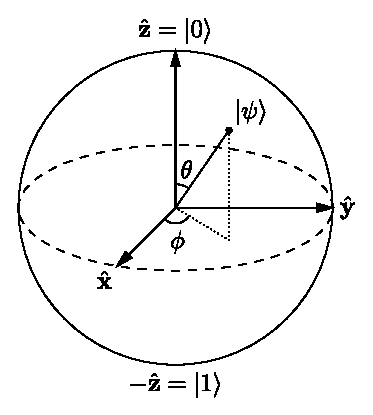
\includegraphics[scale=0.6]{bloch.eps}}
  \caption{Сфера Блоха як представлення квабіта $|\psi\rangle$}
\end{figure}
\end{definition}

\begin{definition} (Машинне слово).
\end{definition}

\begin{definition} (Векторний простір). Множина V називається векторни мпростором над
скалярним полем F, тоді і тільки тоді, коли визначені операції $+ :V \times V \rightarrow V$ (сума векторів)
та $\dot:F\times V\rightarrow V$ (скалярне множення) за наступними властивостями:
i) $(V,+)$ утворюють комутативну групу;
ii) $\lambda |\psi\rangle = |\psi\rangle \lambda$;
iii) $\lambda(\mu|\psi\rangle) = (\lambda\mu)|\psi\rangle$;
iv) $(\lambda+\mu)|\psi\rangle = \lambda|\psi\rangle + \mu|\psi\rangle$;
v) \lambda(|\psi\rangle+|\varphi\rangle) = \lambda|\psi\rangle + \lambda|\varphi\rangle$.
Далі будемо розглядати скалярне поле комплексних чисел $F=C$.
\end{definition}

\begin{definition} (Скалярний добуток).
Функція $\langle\dot|\dot\rangle:V\times V\rightarrow C$ називається скалярним
добутком, тоді і тільки тоді, коли:
i) $\langle\psi|(\lambda\varphi\rangle+\mu|\chi\rangle) = \lambda\langle\psi|\varphi\rangle+\mu\langle\psi|\varphi\rangle$;
ii) $\langle\psi|\varphi\rangle = \langle\varphi|\psi\rangle^*$;
iii) $0 < \langle\psi|\psi\rangle \in \mathbb{R}.
Скалярний добутов визначає норму $\parallel|\psi\rangle\parallel = \sqrt{\langle\psi|psi\rangle} = \paralell\psi\parallel$.

\begin{definition} (Повний векторний простір).
Нехай V векторний простір з нормою $\parallel\dot\parallel$ та $|\psi_n\rangle \in V$
послідовність векторів.
i) $|\psi\rangle$ є послідовністю Коші ттт. $\forall\epsilon>0\exists N>0 : \forall n,m> N, \parallel |\psi_n\rangle - |\psi_{n+1}\rangle\parallel < \epsilon$.
ii) $|\psi\rangle$ сходиться ттт. $\forall\epsilon>0\exists N>0 : \forall n> N, \parallel |\psi_n\rangle - |\psi\rangle\parallel < \epsilon$.
Простір V повний ттт. кожна послідовність Коші сходиться.
\end{defintion}

\begin{definition} (Гільбертів простір).
Повний векторний простір H зі скалярний добутком $\langle\dot|\dot\rangle$ та
відповідною нормою $\parallel\psi\parallel=\sqrt{\langle\psi|\psi\rangle}$ називається Гільбертовим.
\end{definition}

\section{Огляд існуючих мов}

\subsection{QCL}

\subsection{Quantum Lambda}

\section{Висновки}

\bibliographystyle{plain}
\bibliography{quantum}

\end{document}

